
\chapter{Scripting}
\label{ch:scripting}

\section{Introduction}
\label{sec:scripting:introduction}


The development of a powerful scripting system has been continuing for
a number of years now and can now be called operational. The use of a
script was recognised as a perfect way of arranging a display of a
sequence of astronomical events from the earliest versions of
Stellarium and a simple system called \emph{Stratoscript} was
implemented. The scripting facility is Stellarium's version of a
\emph{Presentation}, a feature that may be used to run an astronomical
or other presentation for instruction or entertainment from within the
Stellarium program. The original \emph{Stratoscript} was quite limited in
what it could do so a new Stellarium Scripting System has been
developed.

Since version 0.10.1, Stellarium has included a scripting feature based on
the Qt Scripting
Engine\footnote{\url{http://doc.qt.io/qt-5/qtscript-index.html}}. This
makes it possible to write small programs within Stellarium to produce
automatic presentations, set up custom configurations, and to automate
repetitive tasks. 

As of version 0.14.0 a new scripting engine has reached a level where
it has all required features for usage, however new commands may be
added from time to time. Since version 0.14.0 support of scripts for
the \emph{Stratoscript} engine has been discontinued.

The programming language
ECMAscript\footnote{\url{https://en.wikipedia.org/wiki/ECMAScript}}
(also known as JavaScript) gives users access to all basic ECMAScript
language features such as flow control, variables, string manipulation
and so on.

Interaction with Stellarium-specific features is done via a collection
of objects which represent components of Stellarium itself.  The
various modules of Stellarium, and also activated plugins, can be
called in scripts to calculate, move the scene, switch on and off
display of objects, etc.  You can write text output into text files
with the \command{output()} command.  You can call all public slots
which are documented in the scripting API documentation\footnote{
\url{http://www.stellarium.org/doc/\StelSeries/scripting.html}}.

\section{Script Console}
\label{sec:scripting:console}
It is possible to open, edit run and save scripts using the script
console window. To toggle the script console, press \key{F12}. The
script console also provides an output window in which script
debugging output is visible. 

\section{Includes}
\label{sec:scripting:includes}

Stellarium provides a mechanism for splitting scripts into different
files. Typical functions or lists of variables can be stored in
separate \file{.inc} files and used within other scripts through the
\textbf{include()} command:
\begin{script}
include("common_objects.inc");
\end{script}


\section{Minimal Scripts}
\label{sec:scripting:MinimalScript}
This script prints ``Hello Universe'' in the Script Console log window and into \file{log.txt}:
\begin{script}
core.debug("Hello Universe");
\end{script}

\noindent This script prints ``Hello Universe'' in the Script Console output window and into the file \file{output.txt} 
which you will also find in the user data directory. The absolute path to the file will also be given in \file{log.txt}.
\begin{script}
core.output("Hello Universe");
\end{script}
The file \file{output.txt} will be rewritten on each run of Stellarium. In case you need to save a copy of the current output file to another file, call 
\begin{script}
core.saveOutputAs("myImportantData.txt");
core.resetOutput();
\end{script}

\noindent This script uses the LabelMgr module to display ``Hello Universe'' in red, fontsize 20, on the screen for 3 seconds.
\begin{script}
var label=LabelMgr.labelScreen("Hello Universe", 200, 200, 
                               true, 20, "#ff0000");
core.wait(3);
LabelMgr.deleteLabel(label);
\end{script}

\section{Example: Retrograde motion of Mars}
\label{sec:scripting:RetrogradeMotionOfMars}
A good way begin writing of scripts: set yourself a specific
goal and try to achieve it with the help of few simple steps. Any
complex script can be split into simple parts or tasks, which may solve any
newbie problems in scripting.

Let me explain it with examples.

Imagine that you have set a goal to make a demonstration of a  very
beautiful, but longish phenomenon --- the retrograde motion of the
planet Mars (Fig.~\ref{fig:Mars2005}).

\begin{figure}[tb]
\centering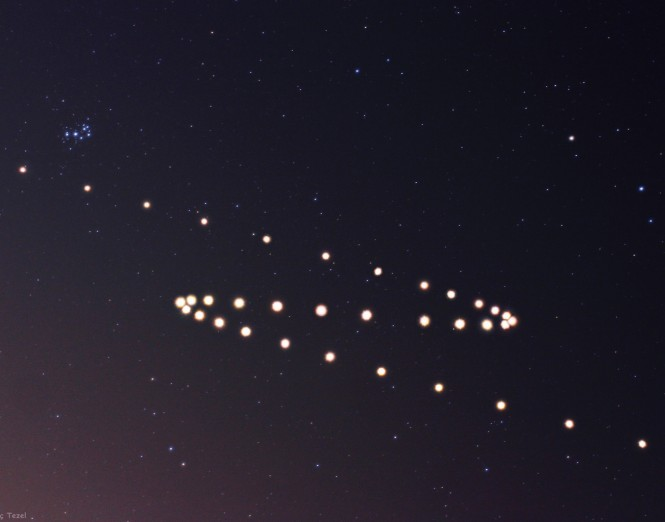
\includegraphics[width=0.8\linewidth]{Mars2005_tezel.jpg}
\caption{Retrograde motion of Mars in 2005. {\small(Credit \& Copyright: Tunc Tezel --- APOD: 2006 April 22 -- Z is for Mars.)}}
\label{fig:Mars2005}
\end{figure}

\subsection{Script header}
Any ``complex'' script should contain a few lines in the first part 
of the file, which contains important data for humans --- the 
name of the script and its description --- and some rules for 
Stellarium. You can even assign default shortcuts in the script header, 
but make sure you assign a key not used elsewhere! The description 
may cover several lines (until the end of the commented header) 
and should therefore be the last entry of the header.

\begin{script}
//
// Name: Retrograde motion of Mars
// Author: John Doe
// License: Public Domain
// Version: 1.0
// Shortcut: Ctrl+M
// Description: A demo of retrograde motion of Mars.
//
\end{script}

\subsection{A body of script}
At the first stage of writing of the script for a demo of 
retrograde motion of Mars we should set some limits for 
our demo. For example we want to see motion of Mars every 
day during 250 days since October $1^{st}$,  2009. 
Choosing a value of field of view and of the coordinates 
of the center of the screen should be done at the this 
stage also. 

Let's add few lines of code into the script after the header 
and run it:
\begin{script}
core.setDate("2009-10-01T10:00:00");
core.moveToRaDec("08h44m41s", "+18d09m13s",1);
StelMovementMgr.zoomTo(40, 1);
for (i=0; i<250; i++)
{
      core.setDate("+ 1 days");
      core.wait(0.2);
}
\end{script}

OK, Stellarium is doing something, but what exactly is it
doing? The ground and atmosphere is enabled and any 
motion of Mars is invisible. Let's add an another few 
lines into the script (hiding the landscape and atmosphere) 
after setting date and time:

\begin{script}
LandscapeMgr.setFlagLandscape(false);
LandscapeMgr.setFlagAtmosphere(false);
\end{script}

The whole sky is moving now --- let's lock it! Add this line 
after previous lines:
\begin{script}
StelMovementMgr.setFlagLockEquPos(true);
\end{script}

It looks better now, but what about cardinal points, 
elements of GUI and some ``glitch of movement''? 
Let's change the script:
\begin{script}
core.setDate("2009-10-01T10:00:00");
LandscapeMgr.setFlagCardinalsPoints(false);
LandscapeMgr.setFlagLandscape(false);
LandscapeMgr.setFlagAtmosphere(false);
core.setGuiVisible(false);
core.moveToRaDec("08h44m41s", "+18d09m13s",1);
StelMovementMgr.setFlagLockEquPos(true);
StelMovementMgr.zoomTo(40, 1);
core.wait(2);
for (i=0; i<250; i++)
{
      core.setDate("+ 1 days");
      core.wait(0.2);
}
core.setGuiVisible(true);
\end{script}

It's better, but let's draw the ``path'' of Mars! Add 
those line before the loop:
\begin{script}
core.selectObjectByName("Mars", false);
SolarSystem.setFlagIsolatedTrails(true);
SolarSystem.setFlagTrails(true);
\end{script}

Hmm\ldots let's add a few strings with info for users (insert 
those lines after the header):
\begin{script}
var color = "#ff9900";
var info = LabelMgr.labelScreen("A motion of Mars", 20, 20, 
           false, 24, color);
var apx = LabelMgr.labelScreen("Setup best viewing angle, FOV 
          and date/time.", 20, 50, false, 18, color);
LabelMgr.setLabelShow(info, true);
LabelMgr.setLabelShow(apx, true);
core.wait(2);
LabelMgr.setLabelShow(apx, false);
\end{script}

Let's add some improvements to display info for users --- 
change in the loop:
\begin{script}
var label = LabelMgr.labelObject("  Normal motion, West to 
            East", "Mars", true, 16, color, "SE");
for (i=0; i<250; i++)
{
	core.setDate("+ 1 days");
	if ((i % 10) == 0)
	{
		var strDate = "Day " + i;
		LabelMgr.setLabelShow(apx, false);
		var apx = LabelMgr.labelScreen(strDate, 20, 
				  50, false, 16, color);
		LabelMgr.setLabelShow(apx, true);
	}
	if (i == 75)
	{
		LabelMgr.deleteLabel(label);
		label = LabelMgr.labelObject("  Retrograde or 
		        opposite motion begins", "Mars", 
		        true, 16, color, "SE");
		core.wait(2);
		LabelMgr.deleteLabel(label);
		label = LabelMgr.labelObject("  Retrograde 
		        motion", "Mars", true, 16, color, 
		        "SE");
	}
	if (i == 160)
	{
		LabelMgr.deleteLabel(label);
		label = LabelMgr.labelObject("  Normal motion 
		        returns", "Mars", true, 16, color, 
		        "SE");
		core.wait(2);
		LabelMgr.deleteLabel(label);
		label = LabelMgr.labelObject("  Normal motion", 
		        "Mars", true, 16, color, "SE");
	}
	core.wait(0.2);
}
\end{script}

\section{More Examples}
\label{sec:scripting:examples}
The best source of examples is the \file{scripts} sub-directory of the
main Stellarium source tree. This directory contains a sub-directory
called \file{tests} which are not installed with Stellarium, but are
nonetheless useful sources of example code for various scripting
features.



% TODO: More examples? 

%%% Local Variables: 
%%% mode: latex
%%% TeX-master: "guide"
%%% End: 
